\chapter{Preliminary} \label{chap: Preliminary}

\section{Use case Wittenstein and BMW}
To get to the point quickly, some prior knowledges will be provided. 

This work is under the ongoing flagship project KI.FABRIK, aims to 
find solutions to enable direct physical interactions between humans and 
machines. The current status of the studies is mainly based on two use 
cases: Wittenstein and BMW use case. 

The Wittenstein gearbox assembly use case mainly involves the cooperation of different 
robots, including a mobile picking robot that collects assembly parts from 
the supermarket cell with a shop list and then puts them into a standard box (KLT). 
After that, the picking robot will move the standard box to the assembly line for 
the assembly task. The assembly tasks are divided into different subtasks for 
multiple assembly robots. After finishing each subtask, the picking robot 
will come again and move the semi-finished product to the next assembly station. 
In case of emergency, teleoperations will be performed to fix the 
errors. 

Similarly, the BMW use case also includes assembly tasks, but for the cockpit 
pre-assembly. Instead of assembling gearbox parts, a more delicate wiring task 
is performed. The production consists of four parts: the pre-assembly of the cover, 
the quality assurance with agent 
assistance and \gls{dt} as a checksum, the fitting of the cover to the cockpit, and 
finally, the quality inspection. All these tasks involve the coworking of 
multiple assembly robots and the assistance of teleoperations. Additionally, 
smart logistics are responsible for delivering parts to 
specific assembly robots. At the same time, a central AI should offer information about the current status of 
the production and synchronize the changes simultaneously. 


\section{Message-based software architecture}

Previous work has already provided an initial consideration of the composition 
of a message-based software architecture for an assembly task with two use cases. 
In the
fig.\ref{fig: Msg-based-SW-architecture} below, different agents are responsible for different sub-tasks in the 
production process. The assignment of a task starts from the customer order. 
The \gls{cda} receives a customized requirement that should be analyzed 
and broken down 
into smaller executable sub-tasks based on its local \gls{db}. Inside the coordinator 
agent, a \gls{paas} will do the rescheduling and dispatching of the customer 
requirements if no matching in local \gls{db} is found. Based on the \gls{paas} 
coordination results and feedback will be given to the customer side. For successful 
task scheduling, the coordinator should be able to check the field-level 
agents for their capabilities. The status checking starts with the transport agent 
and storage agent since both are assigned a task to gather 
assembly parts at the beginning. The sequence of the capability check 
depends on the current robot status. Assume if the storage agent is busy with 
other tasks, the transport agent can receive the task first and wait until 
the storage agent responds, and vice versa. After receiving the assembly parts, the transport 
agent delivers the parts to the wiring (BMW) or assembly agents (Wittenstein) that 
conducts assembly tasks. After the process is executed, the transport 
agent again delivers the gearbox or cockpit back to the product agent, who is 
responsible for the end-product logistics. Once the task execution is 
finished, feedback will be given back to the \gls{cda} to close 
the process. During the production processes, the current robot states will be 
stored in the local database and synchronized with the \gls{dta} and 
then the global \gls{dt}.


\begin{figure}[htb]
    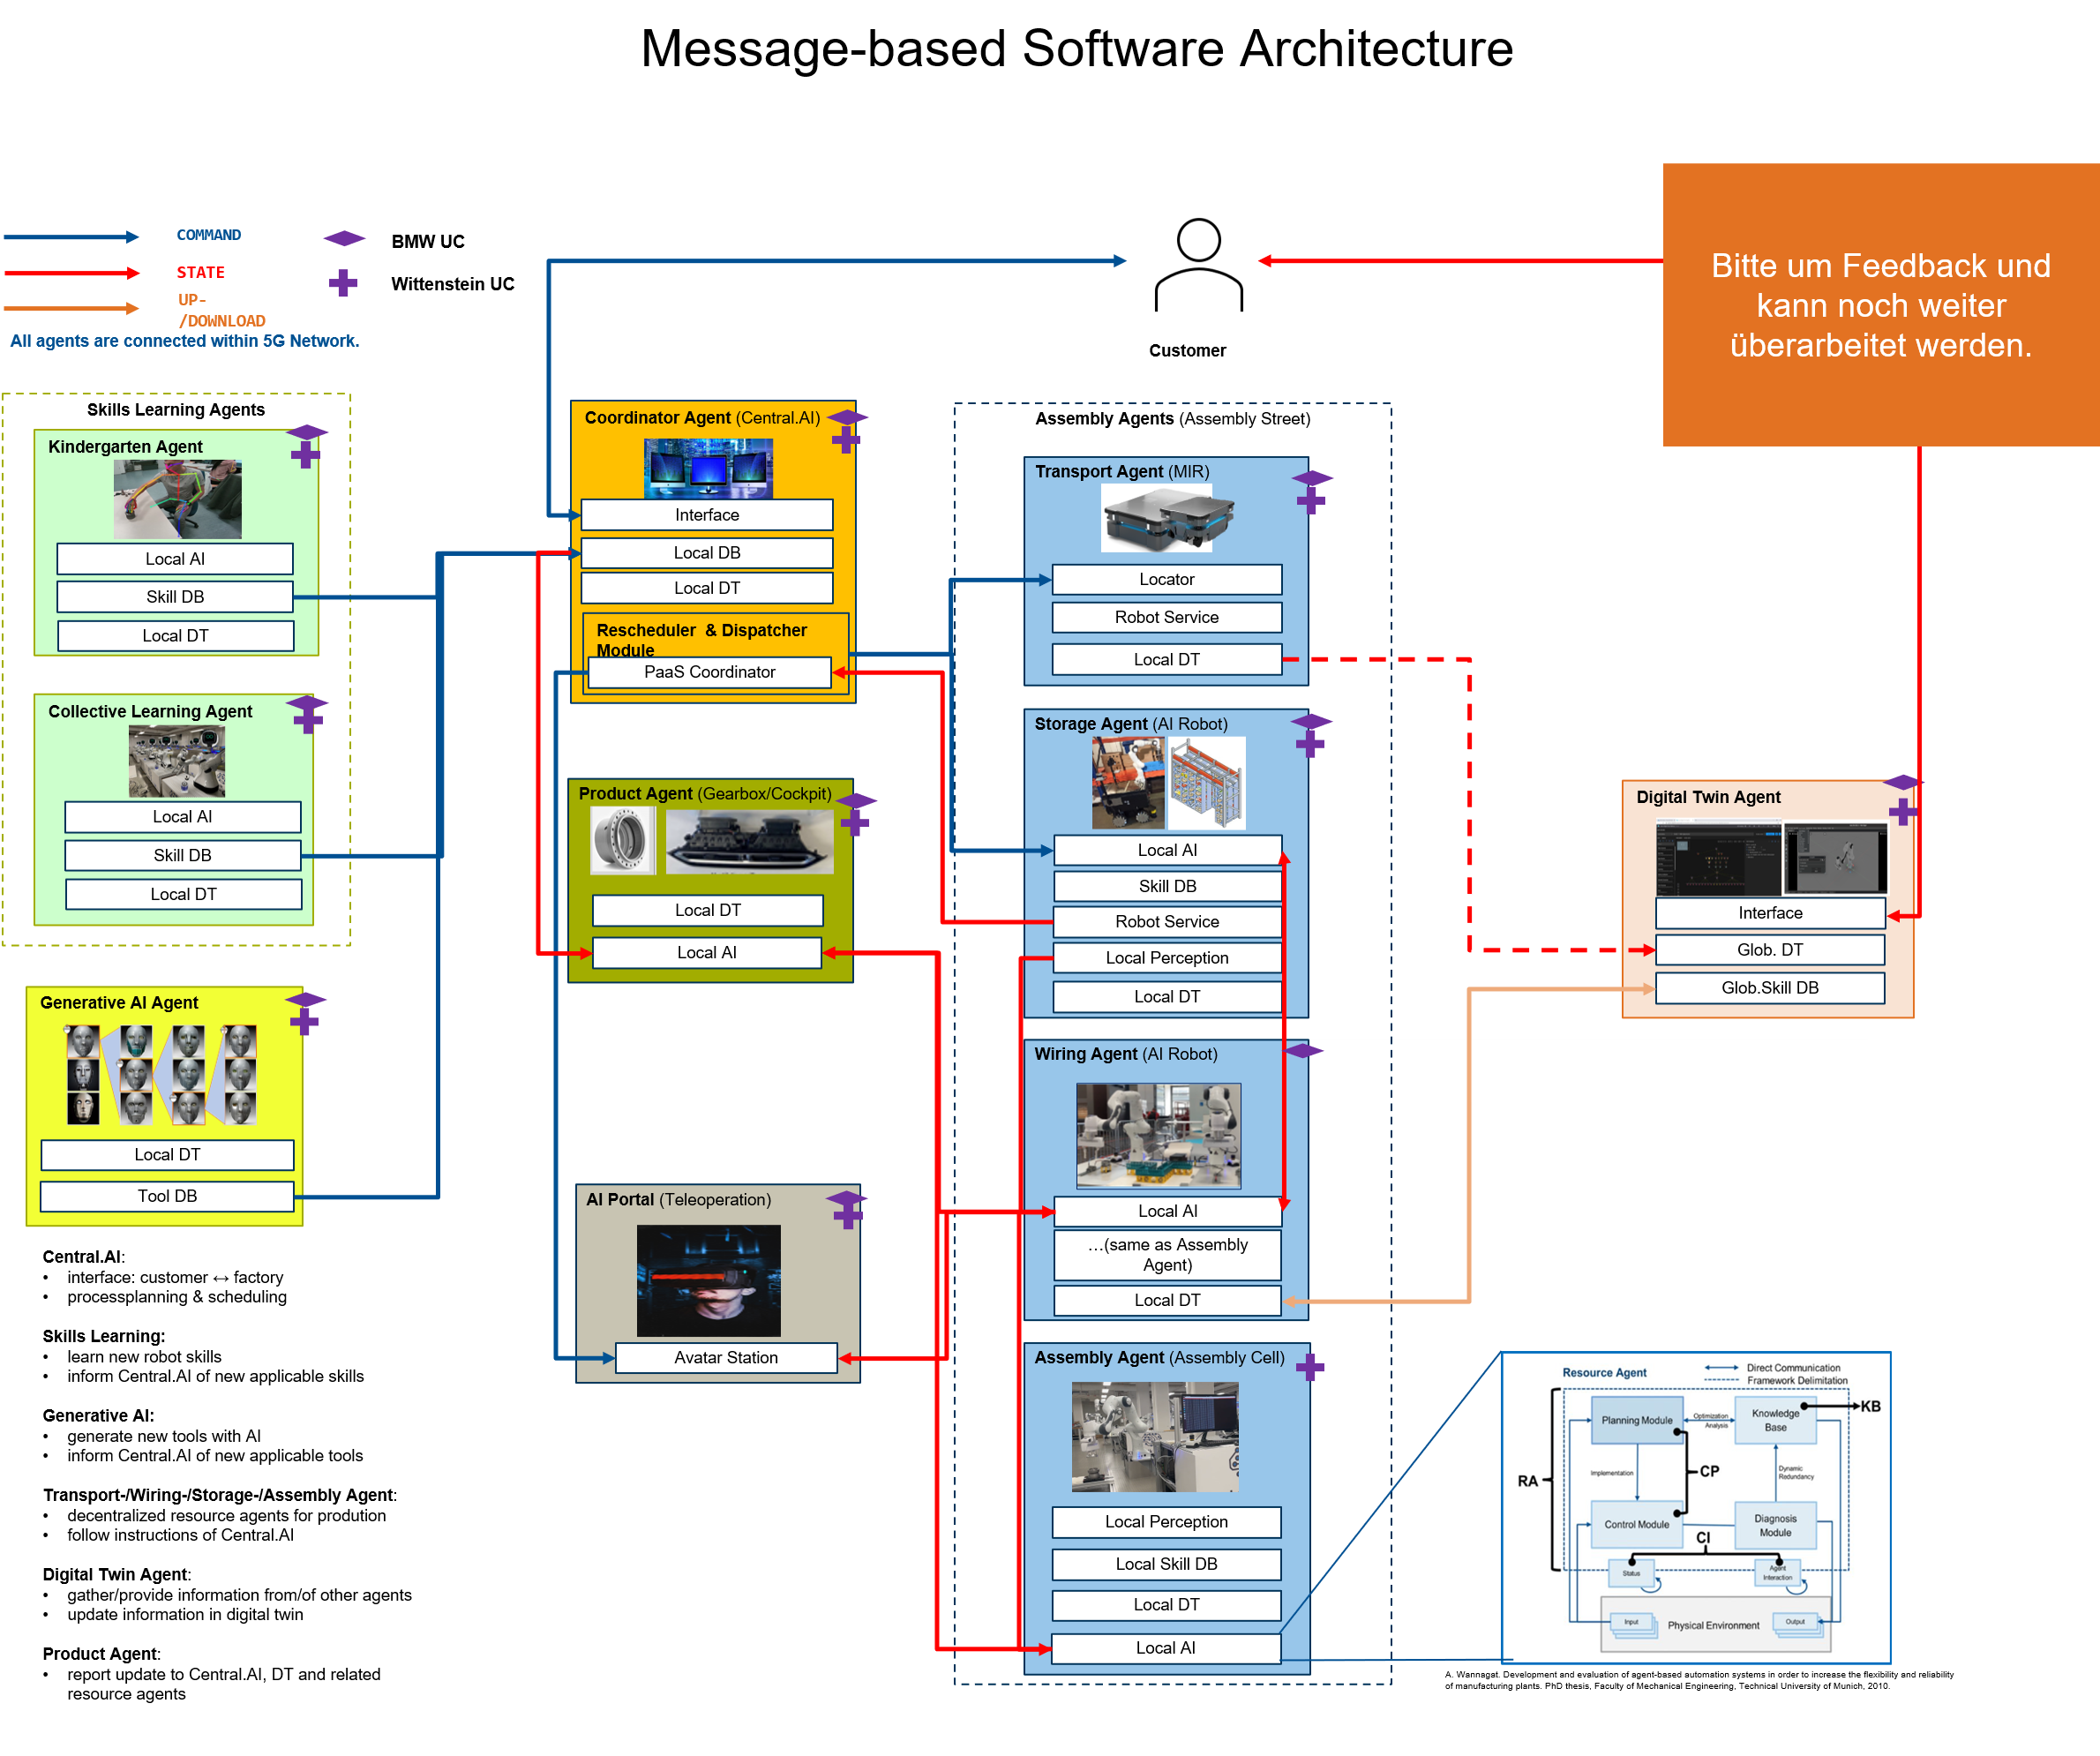
\includegraphics[width=\textwidth]{figures/Prelimilary/Msg-based-Software-Architecture.png}
    \centering
    \caption{Message-based software architecture of two use cases\label{fig: Msg-based-SW-architecture}}
    \end{figure}


Unlike other robot-like systems, the \gls{mas} benefits from the 
cooperation and coordination of multiple agents. More importantly, agents 
are intelligent and can make their own decisions. For example, a transport 
agent can perceive the assembly street for optimized path planning. 
A storage agent can learn to find the shortest path to grasp the parts in 
an optimized sequence. The assembly and wiring agent plans local tasks 
to calculate the optimized assembly and routing trajectories. These 
agent-specific functionalities can be reorganized as different modules, 
based on the wannagat's architecture\cite{wannagat_agent_nodate}, as a 
specification of the local AI in the fig.\ref{fig: Msg-based-SW-architecture}. 


Even though presented, those agents responsible for learning 
and teleoperations are out of the scope of this article. The \gls{mas} here 
only discusses the production processes and their digital mapping.


%\section{Wannagat's architecture with detailed explanation}
